\graphicspath{{fig/model_development/}}

\chapter{Model development}
\label{cha:model_dev}

In this chapter we shall introduce one of the most popular and well-studied
agent-based models in the literature: the Vicsek model. The Vicsek model
represents a simple alignment model in which agents interact with neighbours
within some fixed distance \parencite{vicsek95}. Despite its simplicity, this
model can produce sophisticated dynamics reminiscent of real flocking events
\parencite{ginelli16}. A phase transition from order to disorder is observed as
the amount of noise in the model is regulated \parencite{vicsek12}.

The Vicsek model, like many other agent based models (ABMs)
\parencite{aoki82,couzin02,huth92}, implements a so-called `zonal' interaction
rule. These rules represent discontinuous interactions. With this, the onset of
interaction between individuals is very sensitive to small perturbations in
distances. We consider continuous interaction rules as providing a
biologically-motivated alternative to zonal rules. Such rules ensure
interactions are more robust to small perturbations in distances, but without
the penalty of introducing additional model complexity. We believe that the
introduction of continuous interaction rules represents a step towards
biological realism. 

\section{The Vicsek model}
\label{sec:vicsek_model}

The Vicsek model simulates the movements of $N$ individuals over $T$ time steps
(\cref{fig:vicsek_illustration}). Individuals travel with constant speed $v$,
within a square-cell with periodic boundary conditions and side length $L$. To
initialise a simulation agents are allocated a random position within the cell,
and a random direction of motion. From time $t$ to time $t+1$ agent $i$ updates
its position as:
\begin{equation}
  \label{eq:positional_update}
  \bm{x}_{i, t+1} = \bm{x}_{i, t} + \bm{v}_{i, t},
\end{equation}
where the velocity $\bm{v}_{i,t}$ is constructed to have speed $v$ and
direction of motion $\theta_{i, t+1}$. Updating $\theta_{i,t}$ to $\theta_{i,
t+1}$ models how agents update their directions of motion in light of their
neighbours' movements. The ability of individuals to observe and react to the
movements of their neighbours is assumed to be imperfect, and so a noise term,
in the form of a random directional perturbation, is introduced. In the Vicsek
model noise is considered to be uniformly distributed as $\mathcal{U}(-\eta/2,
\eta/2)$, for some constant $\eta \in [0, 2\pi)$. The directional update of
agent $i$ can then be expressed as a realisation from
\begin{equation}
  \label{eq:vicsek_update}
  \theta_{i, t+1} \given \angmean{\theta}_{i, t}, \eta \sim
                 \mathcal{U}(\angmean{\theta}_{i, t} - \eta/2,
                             \angmean{\theta}_{i, t} + \eta/2),
\end{equation}
where $\angmean{\theta}_{i, t}$ represents the average direction of motion of
agent $i$'s neighbours at time $t$. A weighted circular mean, computed using
the definition of the $\atantwo$ function given in \cref{eq:atantwo}, is used
to compute $\angmean{\theta}_{i, t}$ as:
\begin{equation}
  \label{eq:weighted_interaction}
  \angmean{\theta}_{i, t} = \atantwo\bigg(
      \sum_{j=1}^N \omega_{ij, t} \sin\theta_{j,t},
      \sum_{j=1}^N \omega_{ij, t} \cos\theta_{j,t}
  \bigg).
\end{equation}
With this, the weighting $\omega_{ij, t}$ represents the strength of the
interaction between agent $i$ and agent $j$ at time $t$. In the Vicsek model
agent $i$ interacts with neighbours which are within distance
$r\in\mathbb{R}^+$ of its current position. This interaction can be implemented
with the weighting rule
\begin{equation}
  \label{eq:vicsek_interaction}
  \omega_{ij,t} =
  \begin{cases}
    1 & \text{ if } d_{ij, t} \leq r,\\
    0 & \text{ otherwise,}
  \end{cases}
\end{equation}
where $d_{ij,t}$ is the Euclidean-distance between the positions of agent $i$
and agent $j$ at time $t$:
\begin{equation*}
  d_{ij,t} = \sqrt{(x_{j,t} - x_{i,t})^2 + (y_{j,t} - y_{i,t})^2}.
\end{equation*}

The interaction rule implemented in the Vicsek model represents a discontinuous
interaction, as the interaction kernel is very sensitive to small perturbations
in distances. More formally, this discontinuity can be shown by considering the
value of $\omega_{ij, t}$ as $d_{ij,t}$ approaches $r$ from above and below. As
$d_{ij,t}$ approaches $r$ from above we realise the limit $\lim_{d_{ij,t}
\rightarrow r^+} \omega_{ij,t} = 0$. Conversely, as $d_{ij,t}$ approaches $r$
from below we observe $\lim_{d_{ij,t} \rightarrow r^-} \omega_{ij,t} = 1$. As
the weighting tends to different values as the limit of $d_{ij,t}=r$ is
approached, we see that there is a discontinuity at $d_{ij,t}=r$. This
weighting rule and its resulting discontinuity are visualised in
\cref{fig:vicsek_weight}.

The Vicsek model was inspired by models of ferromagnetism. In these models
particles align spin states with neighbouring particles. Although a
discontinuous interaction rule may be appropriate for such models, it is not
clear whether the hard cut-off imposed by the interaction radius $r$ is
appropriate for biological systems. Later, we shall introduce models
implementing continuous interaction rules as a biologically-motivated
alternative.

\textcite{vicsek95} used this model to examine polarisation of simulated flocks
as the magnitude of the noise ($\abs{\eta}$) was varied. The polarisation of a
flock at time $t$---sometimes referred to as its alignment---was quantified by
the absolute value of the normalised velocity of the flock:
\begin{equation}
  \label{eq:alignment}
  v_{a,t} = \frac{1}{Nv} \abs{\,\sum_{i=1}^N \bm{v}_{i,t}\,}.
\end{equation}
A flock moving incohesively at time $t$, with individual members directed
randomly, has polarisation $v_{a,t}\approx0$. Conversely, a highly polarised
flock in which all members are moving in the same direction at time $t$ has an
alignment $v_{a,t}\approx1$. As the amount of noise in a simulation is
increased flocks are observed to transition from an ordered $v_{a,t}\approx1$
state to a disordered $v_{a,t}\approx0$ state. For a fixed flock density,
smaller flocks are observed to be more resistant to noise than larger flocks.

\begin{figure}[tb]
  \begin{subfigure}[b]{0.5\textwidth}
    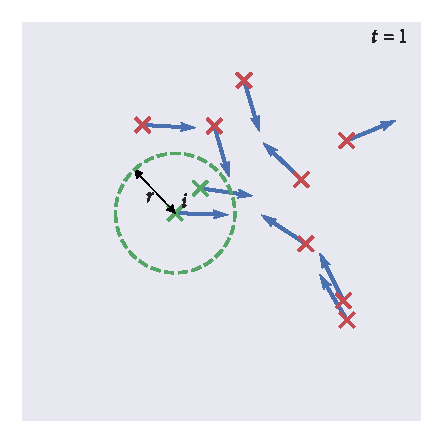
\includegraphics{vicsek_simulation_1.pdf}
  \end{subfigure}%
  \begin{subfigure}[b]{0.5\textwidth}
    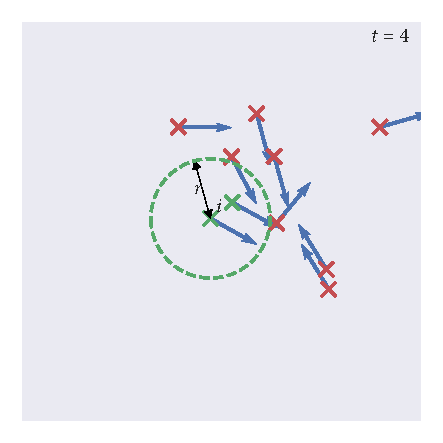
\includegraphics{vicsek_simulation_4.pdf}
  \end{subfigure}
  \begin{subfigure}[b]{0.5\textwidth}
    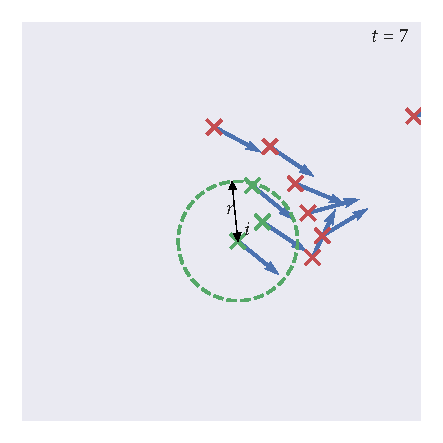
\includegraphics{vicsek_simulation_7.pdf}
  \end{subfigure}%
  \begin{subfigure}[b]{0.5\textwidth}
    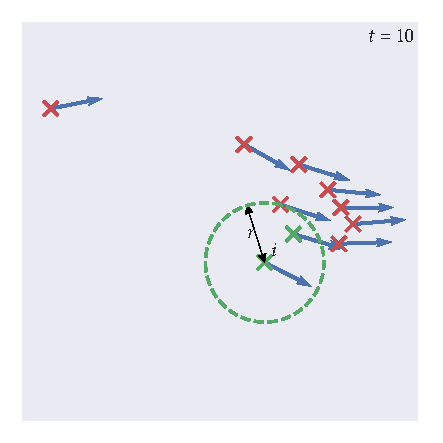
\includegraphics{vicsek_simulation_10.pdf}
  \end{subfigure}
  \caption{Visualisations from a simulation of the Vicsek model. At time
    $t=1$, $N=10$ agents are assigned random positions within a square-cell
    of side length $L=1$. Initially, the directions of motion of
    individuals are realised from a $\mathcal{U}(-\pi, \pi)$ distribution.
    Between time steps agents move with speed $v=0.03$, and update
    directions according to \cref{eq:vicsek_update}, with $\eta=\pi/16$.
    The interaction zone of agent $i$ is illustrated throughout the
    simulation by a circle of radius $r$ centred at $\bm{x}_{i,t}$. The
    positions of neighbours within agent $i$'s interaction zone are
    visualised with a green cross. Individuals which lie outside of agent
    $i$'s interaction zone have their positions denoted by a red cross.}
  \label{fig:vicsek_illustration}
\end{figure}

\subsection{Stochasticity}

Inspired by models of interacting particles, the uniformly distributed noise
implemented in simulations of the Vicsek model is analogous to temperature in a
physical system. However, it is not clear whether this distribution is a
reasonable choice for biologically-motivated systems. In some of the literature
authors instead assume that noise is normally distributed \parencite{couzin02}.
In this case an agent's directional update typically takes the form:
\begin{equation*}
  \label{eq:normal_update}
  \theta_{i,t+1} \given \angmean{\theta}_{i,t}, \sigma_Y \sim
      \mathcal{N}(\angmean{\theta}_{i,t}, \sigma_Y).
\end{equation*}

Given that the $\theta_{i,t}$ represent circular quantities, it is not clear
whether a choice of normally distributed noise is appropriate. Consider that
the normal distribution has infinite support, yet $\theta_{i,t}\in[-\pi,\pi)$
for $i=1,\ldots,N$ and $t=1,\ldots,T$. The von Mises distribution is a
continuous probability distribution on the circle, and so potentially
represents a more appropriate noise structure. However, we observe that when
the magnitude of the noise is small, the von Mises distribution can be
approximated by a normal distribution, as shown in \cref{sec:von_mise}, and so
offers no more flexibility than normally distributed noise.

The Student's $t$-distribution allows more weight in its tails than the normal
distribution. As the degrees of freedom of the Student's $t$-distribution tends
to infinity, the distribution converges to a normal distribution with location
$\mu$ and scale $\sigma_Y$. As such, the Student's $t$-distribution represents
a more flexible noise structure than the normal distribution.

Throughout this work we shall consider that the noise experienced by
individuals is distributed according to some generalised Student's
$t$-distribution with $\nu$ degrees of freedom and scale $\sigma_Y$. In this
situation, the directional update of agent $i$ is given as:
\begin{equation}
  \label{eq:students_update}
  \theta_{i,t+1} \given \angmean{\theta}_{i,t}, \nu, \sigma_Y \sim
     t_{\nu}(\angmean{\theta}_{i,t}, \sigma_Y).
\end{equation}
Although the Student's $t$-distribution represents a more flexible noise
structure, it also comes at the cost of model complexity: with the introduction
of the degrees of freedom $\nu$ as an additional model parameter.

\subsection{Boundary conditions}

Recall that simulations of the Vicsek model take place in a square-cell with
periodic boundary conditions and side-length $L$. In this way the density of a
cell remains constant throughout a simulation. However, implementing periodic
boundary conditions when we attempt to mimic real flocking events is clearly
inappropriate. Instead, we shall consider simulations to take place in the
unrestricted continuous domain represented by $\mathbb{R}^2$. On top of
realism, performing simulations in this unrestricted domain allows more
informative visualisations of the resulting data, as in
\cref{fig:example_traj}. Here we are able to visualise the positions of agents
throughout a simulation in a single graphic. Trajectory plots of simulations
taking place in periodic cells can be difficult to interpret, as it is not easy
to visually track individuals as they cross the periodic boundary.

\begin{figure}[tb]
  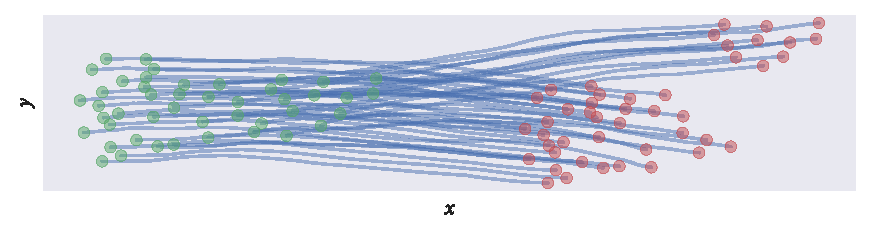
\includegraphics{example_traj_plot.pdf}
  \caption{A trajectory plot representing the movements of $N=45$ agents
    moving through the unrestricted continuous domain $\mathbb{R}^2$.
    Agents are initially positioned at the locations represented by the red
    markers. The model is simulated for $200$ time steps. The green markers
    represent the positions of agents at the end of a simulation. Blue lines
    represent the trajectories of motion of individual agents throughout the
    simulation.}
    \label{fig:example_traj}
\end{figure}

\section{Development}

Although we shall consider variations on the standard Vicsek model, we shall
leave most aspects of this model unchanged. In the following models, agents
shall always update their positions as was seen in \cref{eq:positional_update}.
Similarly, agents will always update their directions of motion according to
\cref{eq:students_update,eq:weighted_interaction}. In fact, all our variations
on the standard Vicsek model shall be made by manipulating the computation of
the weighting $\omega_{ij,t}$. Recall that $\omega_{ij,t}$ represents the
strength of the interaction between agent $i$ and agent $j$ at time $t$.
Varying the form of $\omega_{ij,t}$ allows us to investigate how the behaviour
of a neighbour influences a flock member.

\subsection{The Null model}
\label{sec:null_model}

In later chapters we fit a number of different models to data. We
then assess the predictive performance of these models. Model
performance is assessed by the ability to explain the directional changes
of individuals. Simple models are favoured over complex models. In making
such comparisons, it can be useful to have a baseline with which to compare all
candidate models. It is with this intention which we introduce the Null model.

In the Null model there are no interactions between flock members. All
directional changes are attributed to random noise. The Null model implements
directional updates as in \cref{eq:students_update}, with location
$\angmean{\theta}_{i,t}$ computed from \cref{eq:weighted_interaction} with
weighting $\omega_{ij,t}=\delta_{ij}$, where $\delta_{ij}$ is the Kronecker
delta:
\begin{equation*}
  \delta_{ij} =
  \begin{cases}
    1 & \text{if } i=j \\
    0 & \text{otherwise.}
  \end{cases}
\end{equation*}
This ensures that agents effectively ignore all their neighbours, and update
their directions simply as $\theta_{i,t+1} \given \theta_{i,t}, \nu, \sigma_Y
\sim t_\nu(\theta_{i,t}, \sigma_Y)$.

\subsection{Continuous interaction models}

We have observed that the interaction rule implemented in the Vicsek model
exhibits a discontinuity. This discontinuity raises two concerns. The
biological realism of an interaction rule implementing a hard cut-off is
questionable. Secondly, the ability to fit such a model to data is potentially
problematic: exploring the sample space of a discontinuous target distribution
can be difficult.

Such concerns can be addressed by considering variations of the Vicsek model in
which continuous interaction rules are implemented, as these arguably represent
more biologically realistic behaviours. In addition to this, the MCMC
algorithms used to draw samples from our posterior beliefs are found to be
better behaved for the models implementing continuous interaction rules.

\begin{figure}[tb]
  \begin{subfigure}[b]{0.5\textwidth}
    \caption{Vicsek weighting}
    \label{fig:vicsek_weight}
    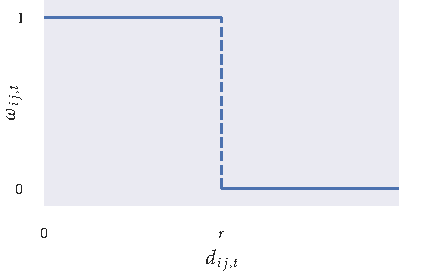
\includegraphics{vicsek_weighting.pdf}
  \end{subfigure}%
  \begin{subfigure}[b]{0.5\textwidth}
    \caption{Power-law weighting}
    \label{fig:power_weight}
    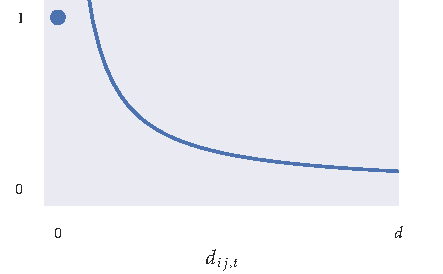
\includegraphics{power_weighting.pdf}
  \end{subfigure}\\
  \begin{subfigure}[b]{0.5\textwidth}
    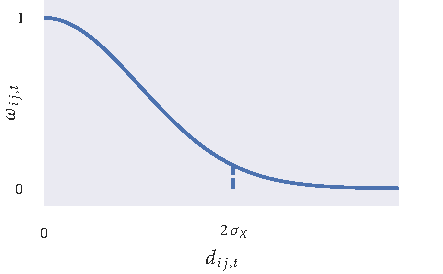
\includegraphics{gaussian_weighting.pdf}
    \caption{Gaussian weighting}
    \label{fig:gauss_weight}
  \end{subfigure}%
  \begin{subfigure}[b]{0.5\textwidth}
    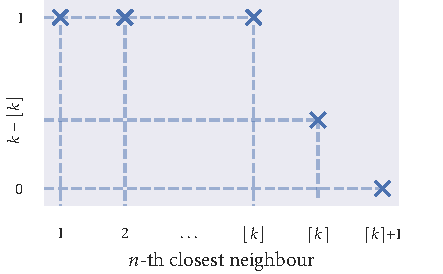
\includegraphics{topological_weighting.pdf}
    \caption{Topological weighting}
    \label{fig:top_weight}
  \end{subfigure}
  \caption{Visualisations of the weighting rules investigated in this thesis.
    \subref{fig:vicsek_weight} The interaction implemented in the Vicsek model,
    parameterised by the interaction radius $r$, exhibits a discontinuity
    (\cref{eq:vicsek_interaction}).
    \subref{fig:power_weight} In the power-law weighted model the strength of
    the interaction between individuals decays as a power-law relationship with
    their distance apart, parameterised by decay rate $\alpha$
    (\cref{eq:power_law_interaction}).
    \subref{fig:gauss_weight} The
    strength of interaction between individuals is controlled by a Gaussian
    kernel with standard deviation $\sigma_X$
    (\cref{eq:gaussian_interaction}).
    \subref{fig:top_weight} A realisation of
    a topological interaction which allows contributions from partial neighbours
    (\cref{eq:top_interaction}).}
  \label{fig:weighting_rules}
\end{figure}

Metric models, of which Vicsek is an example, implement weighting rules which
are explicitly distance-dependant. Here we shall motivate two novel metric
interaction rules. We propose that these represent intuitive and biologically
realistic rules. \cref{fig:weighting_rules} visualises the interaction rule of
Vicsek, alongside the metric models introduced.

\subsubsection{Power-law interaction}

A power-law relationship between two quantities occurs when a relative
change in one quantity results in a proportional change in the other.
Power-law relationships are found frequently in physical and biological
systems, and so represent a natural choice of interaction rule to investigate.

For the power-law weighted model we assume that the interaction strength
between individuals decays as some power-law with their distance
apart:
\begin{equation}
  \label{eq:power_law_interaction}
  \omega_{ij,t} =
  \begin{cases}
    1                  & \, \text{if } d_{ij,t} = 0, \\
	d_{ij,t}^{-\alpha} & \, \text{otherwise}.
  \end{cases}
\end{equation}
The interaction of the Vicsek model is parameterised by the radius $r \geq 0$.
Here the interaction is parameterised by some $\alpha\in\mathbb{R}^+$. The
parameter $\alpha$ controls the rate at which the interaction strength between
individuals decays. 

In this model, the closer a neighbour to agent $i$, the more influence it has
over agent $i$'s behaviour. Conversely, the further away a neighbour is from
the position of agent $i$, the less influence it has on agent $i$'s movements.
The rate at which influence decays is controlled by the value of $\alpha$.
Small values of $\alpha$ represent a more gradual decay of influence with
distance, whereas large values of $\alpha$ correspond to a weighting which
decays rapidly. This weighting rule is visualised in \cref{fig:power_weight}.

This interaction rule, although continuous for $d_{ij,t} > 0$, still exhibits a
discontinuity at $d_{ij,t}=0$. However, in the flocking events which we will
fit this model to we observe $d_{ij,t}\gg0$ $\forall i \neq j$, and so this
discontinuity will not pose an issue during the fitting process.

\subsubsection{Gaussian interaction}

Similar to the power-law weighted model, in the Gaussian weighted model the
influence which neighbour $j$ exerts over agent $i$ is inversely proportional
to their distance apart; the \emph{further} away a neighbour the \emph{less}
influence it exerts. The Gaussian weighted interaction is continuous over all
$d_{ij,t}$, and can be expressed as:
\begin{equation}
  \label{eq:gaussian_interaction}
  \omega_{ij,t} =
	\frac{1}{\sqrt{2\pi\sigma_X^2}}
	e^{-\frac{1}{2}\big(\frac{d_{ij,t}}{\sigma_X}\big)^2}.
\end{equation}
This rule is illustrated in \cref{fig:gauss_weight}.

From \cref{eq:gaussian_interaction} the parameter $\sigma_X$ can be seen to
control the length-scale over which interaction takes place. Small values of
$\sigma_X$ represent a weighting function which is very peaked around agent
$i$'s position. As $\sigma_X \rightarrow \infty$ the weighting approaches a
schema in which all neighbours in the flock are given the same weight. This
limiting behaviour is equivalent to that of Vicsek as $r\rightarrow\infty$, and
the power-law weighted model as $\alpha\rightarrow0$.

Although the Gaussian model implements a similar interaction kernel to that of
the power-law weighted model, there remains differences in their functional
forms. Most notably the power-law interaction represents a convex weighting
function, whereas the Gaussian interaction is a concave weighting
(\cref{fig:weighting_rules}). The Gaussian model also has some inherent length
scale, expressed by the parameter $\sigma_X$, whereas the power-law weighted
interaction is scale-free.

\subsection{Topological models}

Topological rules represent a different type of interaction to metric rules.
Here, agents interact with their $k\in\mathbb{N}$ nearest neighbours,
regardless of their distance apart. This interaction rule was motivated by
simulations which suggested that flocks implementing topological rules were
more resistant to perturbations, such as those by predators, than those
implementing metric rules \parencite{ballerini08,camperi12,ginelli10}. As such,
it was argued that topological interaction rules offer an evolutionary
advantage to flocks over metric interaction rules. It was also posed that the
cognitive limits of individuals puts some upper bound on the number of
neighbours which agents can interact with at any one time
\parencite{giardina08,nieder05}.

Whilst retaining the form of the topological rule, we look to relax the
constraint that agents may only interact with some \emph{integer} number of
closest neighbours. Instead, we allow an agent to interact with some
$k\in\mathbb{R}^+$ nearest neighbours. This allows partial neighbours, which
may make some lesser contribution to an agent's behaviour. An additional
benefit of this more flexible interaction structure is given by the observation
that real-valued parameters are typically easier to infer from data than
discrete parameters.

For some $k\in\mathbb{R}^+$ we say that each agent gives weighting $1$ to its
$\floor{k}$ nearest neighbours, weighting $k - \floor{k}$ to its $\ceil{k}$-th
nearest neighbour, and weighting $0$ to all other agents, where $\floor{\cdot}$
and $\ceil{\cdot}$ are the floor and ceiling function respectively. More
concisely, we can express this as the weighting
\begin{equation}
  \label{eq:top_interaction}
  \omega_{ij,t} =
  \begin{cases}
    1           & \, \text{if } d_{ij, t} \leq \min_j(d_{ij,t},\, \floor{k}), \\
    k-\floor{k} & \, \text{if } d_{ij, t} = \min_j(d_{ij,t},\, \ceil{k}),     \\
    0           & \, \text{otherwise,}
  \end{cases}
\end{equation}
where $\min_j(d_{ij,t},\, k)$ is the distance to agent $i$'s $k$-th closest
neighbour at time $t$. This weighting rule is illustrated in
\cref{fig:top_weight}.

\subsection{Intra-flock variation}

In all the model variations considered thus far, there has been no allowance
for behavioural or biological variation within flocks. That is, presented with
the same circumstances, all of our agents would behave identically. This is
despite our understanding of the importance of biological variation in nature.

Within a single flock, we may reasonably expect there to be variation in the
age, cognitive ability, social standing and physical attributes of the
individuals. Naturally then, it seems reasonable to suggest that if the
attributes of individuals may vary, then their behavioural responses to a
particular set of circumstances may vary too. This is in keeping with the
observation that the orientation abilities of migrating raptors is age
dependent \parencite{thorup03}.

Models allowing intra-flock variation have been considered before. Particularly
impactful was the work of \textcite{couzin05}, which simulated flocks of
individuals partitioned into a group of leaders and a group of followers. The
two groups interacted according to different behavioural rules. Followers
sought only to amend their directions in response to the movements of their
neighbours. Whereas leaders balanced their desire to interact with neighbours
and their desire to move in a particular direction (for example, toward a
migratory of foraging goal).

Instead of dividing agents into distinct behavioural categories, we permit a
range of behavioural responses by allowing interaction and noise parameters to
vary between individuals. Some agents may be more or less susceptible to noise
than others. Consider then that agent $i$ experiences noise distributed
according to a generalised Students $t$-distribution with $\nu$ degrees of
freedom and scale $\sigma_{Y_i}$. Agent $i$'s directional update is then given
as
\begin{equation*}
  \theta_{i,t+1} \given \angmean{\theta}_{i,t}, \nu, \sigma_{Y_i} \sim
    t_{\nu}(\angmean{\theta}_{i,t}, \sigma_{Y_i}).
\end{equation*}

In addition to allowing noise parameters to vary within a flock, we also seek
to allow interaction parameters to vary within a flock. In the case of Vicsek,
agent $i$ would then interact with neighbours positioned within distance $r_i$.
This corresponds to the weighting rule:
\begin{equation}
    \omega_{ij,t} =
    \begin{cases}
        1 & \text{ if } d_{ij, t} \leq r_i,\\
        0 & \text{ otherwise.}
    \end{cases}
\end{equation}
A similar allowance can be made for the power-law weighted, Gaussian weighted
and topological models considered earlier.

\subsubsection{Imposing hierarchy}
\label{ssec:hier_mod}

Rather than considering the individual interaction and noise parameters as
completely unrelated, we can consider them as being realisations from some
population-level distribution. Hierarchical models allow us to incorporate this
extra level of structure into our models.

Hyperparameters are introduced as parameters of the population-level
distribution. Hyperpriors are then specified to reflect the practitioner's
prior beliefs about likely values of the hyperparameters.

The noise and interaction parameters in our models are all strictly positive,
and not bounded above. As such, we shall assume that the population
distributions for these parameters follow some gamma distribution. Consider,
for example, that the noise parameters $\sigma_{Y_i}$ are distributed according
to a gamma distribution with shape $\alpha_Y$ and rate $\beta_Y$. More
concisely, we consider our noise parameters as being distributed according to
\begin{equation}
    \label{eq:noise_hier}
    \sigma_{Y_i}\given\alpha_Y,\beta_Y \sim \Ga(\alpha_Y, \beta_Y).
\end{equation}
Our hyperparameters here are $\alpha_Y$ and $\beta_Y$. The practitioner is then
required to specify hyperpriors: their prior beliefs about likely values for
$\alpha_Y$ and $\beta_Y$. It can be hard to get an intuitive feel for plausible
values for the shape and rate parameters, and so we shall instead
re-parameterise our population-level distribution in terms of the mean and
variance. Consider that the mean and variance of the gamma distribution can be
computed as $m_Y = \alpha_Y / \beta_Y$ and $v_Y = \alpha_Y/\beta_Y^2$
respectively. From these two relations it can be seen that $\alpha_Y = m_Y^2 /
v_Y$ and $\beta_Y = m_Y / v_Y$. \cref{eq:noise_hier} can then be re-expressed
as:
\begin{equation}
    \label{eq:sigma_Y_hierarchy}
    \sigma_{Y_i}\given m_Y, v_Y \sim \Ga\bigg(\frac{m_Y^2}{v_Y},
                                              \frac{m_Y}{v_Y}\bigg).
\end{equation}
This parameterisation allows the practitioner to specify their hyperpriors over
the mean and variance of the distribution, instead of the shape and rate. The
hope is that this will give the practitioner a more intuitive feel for likely
values of the hyperparameters.

Population-level distributions are specified in a similar way for the
interaction parameters of the Vicsek weighting, power-law weighting, Gaussian
weighting and topological models:
\begin{align}
    r_i &\given m_r, v_r  \sim \Ga\bigg(\frac{m_r^2}{v_r}, \frac{m_r}{v_r}\bigg)\\
    \alpha_i &\given m_{\alpha}, v_{\alpha}  \sim
        \Ga\bigg(\frac{m_{\alpha}^2}{v_{\alpha}}, \frac{m_{\alpha}}{v_{\alpha}}\bigg)\\
    \sigma_{X_i} &\given m_X, v_X  \sim \Ga\bigg(\frac{m_X^2}{v_X}, \frac{m_X}{v_X}\bigg)
    \label{eq:sigma_X_hierarchy}\\
    k_i &\given m_k, v_k  \sim \Ga\bigg(\frac{m_k^2}{v_k}, \frac{m_k}{v_k}\bigg)
\end{align}

\section*{Conclusions}

In this chapter we introduced a model developed by \textcite{vicsek95}. This
work received much attention in the following literature, and many studies were
made of its simulations and results. We also considered some of the biological
shortcomings of this model, and proposed alterations to address them.

To compare the predictive performance of variations on the Vicsek model we
introduced a null model. This model implements no interaction rules, and
direction changes are attributed entirely to noise. We also introduced models
implementing continuous interaction rules, under considerations of biological
realism. Continuous variations of both metric and topological models were
introduced.

Variations on these models were considered in which biological and behavioural
variation between individuals is allowed; again motivated by considerations of
biological-realism. Population-level variation was modeled by a hierarchical
structure, with hyperparameters introduced to parameterise the population-level
distributions.

